\subsection{Sensitivity Analysis With Front-end Processors}
From Chapter $2$, we know the speedup is :
$$Speedup = \frac{T_{f, 0}}{T_{f, n}}= \frac{\omega T_{cp}}{\alpha_{0}\omega T_{cp}} = \frac{1}{\alpha_{0}} = \left |-\det A \right |$$.
\subsubsection{Data Injection On The Corner Processor}
The simulation result of sensitivity analysis of $2*n$ regular mesh \Fig{2t10} is as follows:
\begin{figure}[!ht]
\centering
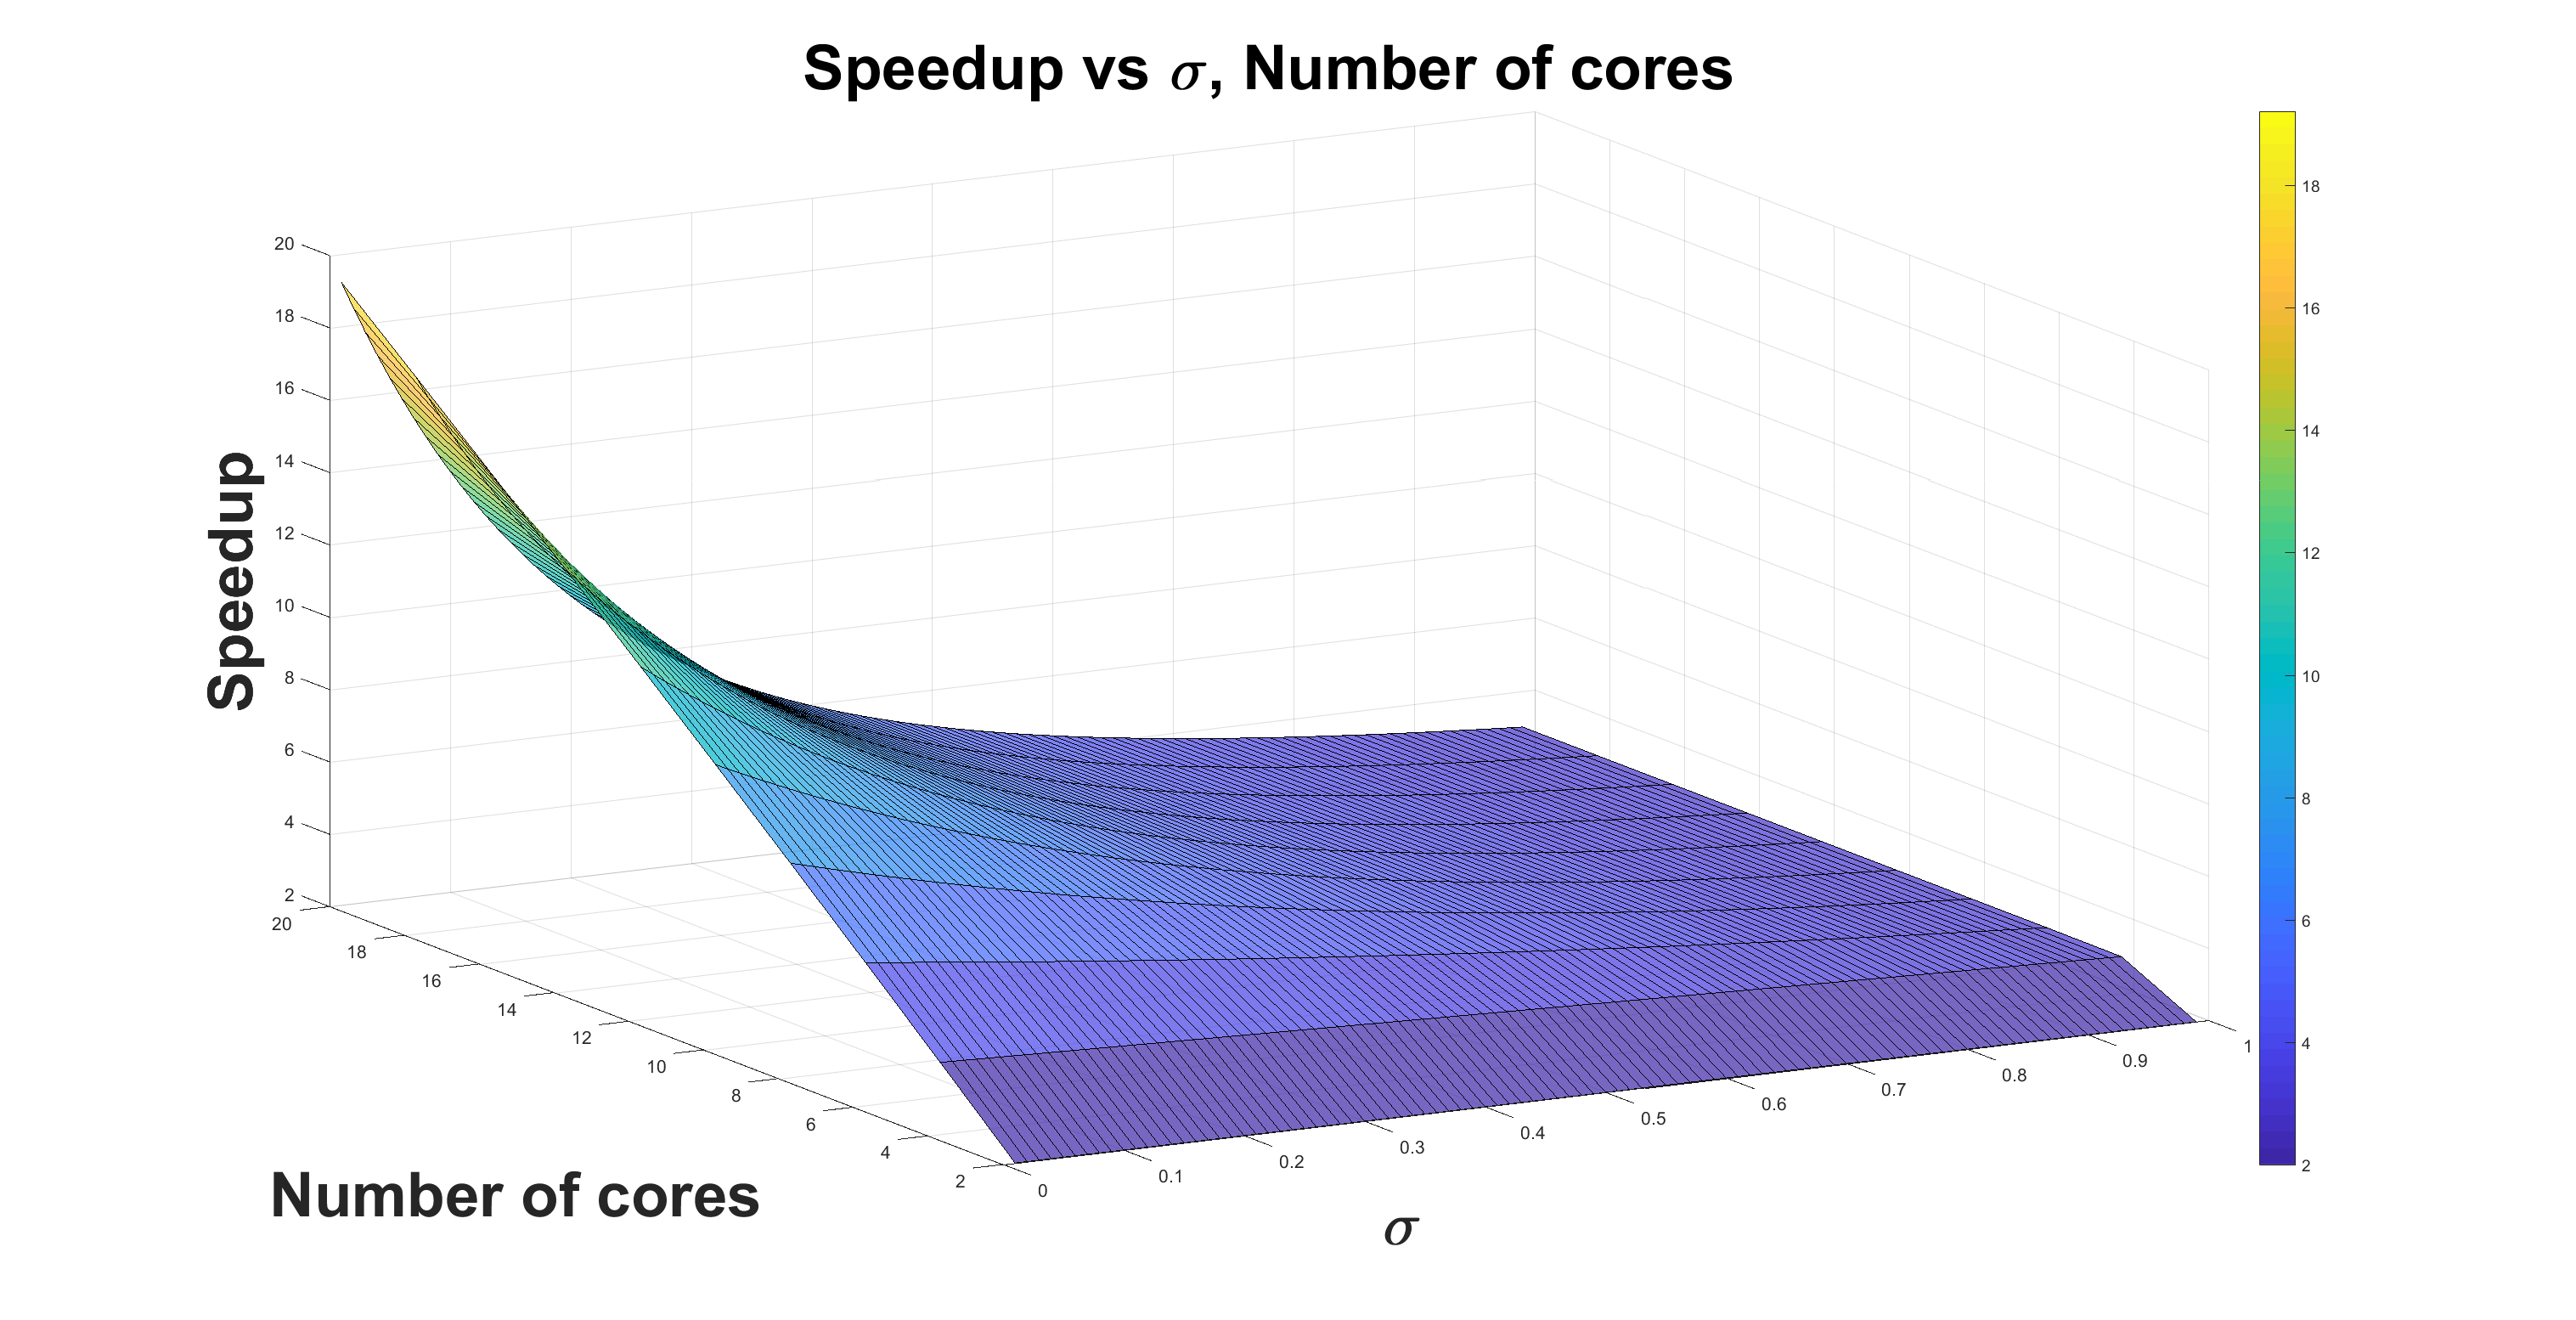
\includegraphics[width=1\columnwidth]{figure/sa2t10c.eps}
\caption{Sensitivity analysis result of 2*10 regular mesh result}
\label{fig:sa2t10c}
\end{figure}

\newpage
\subsubsection{Data Injection On The Boundary Processor}
Talking to \Fig{3t8}, the data injection happens on boundary processor $P_{2}$. 
\begin{figure}[!ht]
\centering
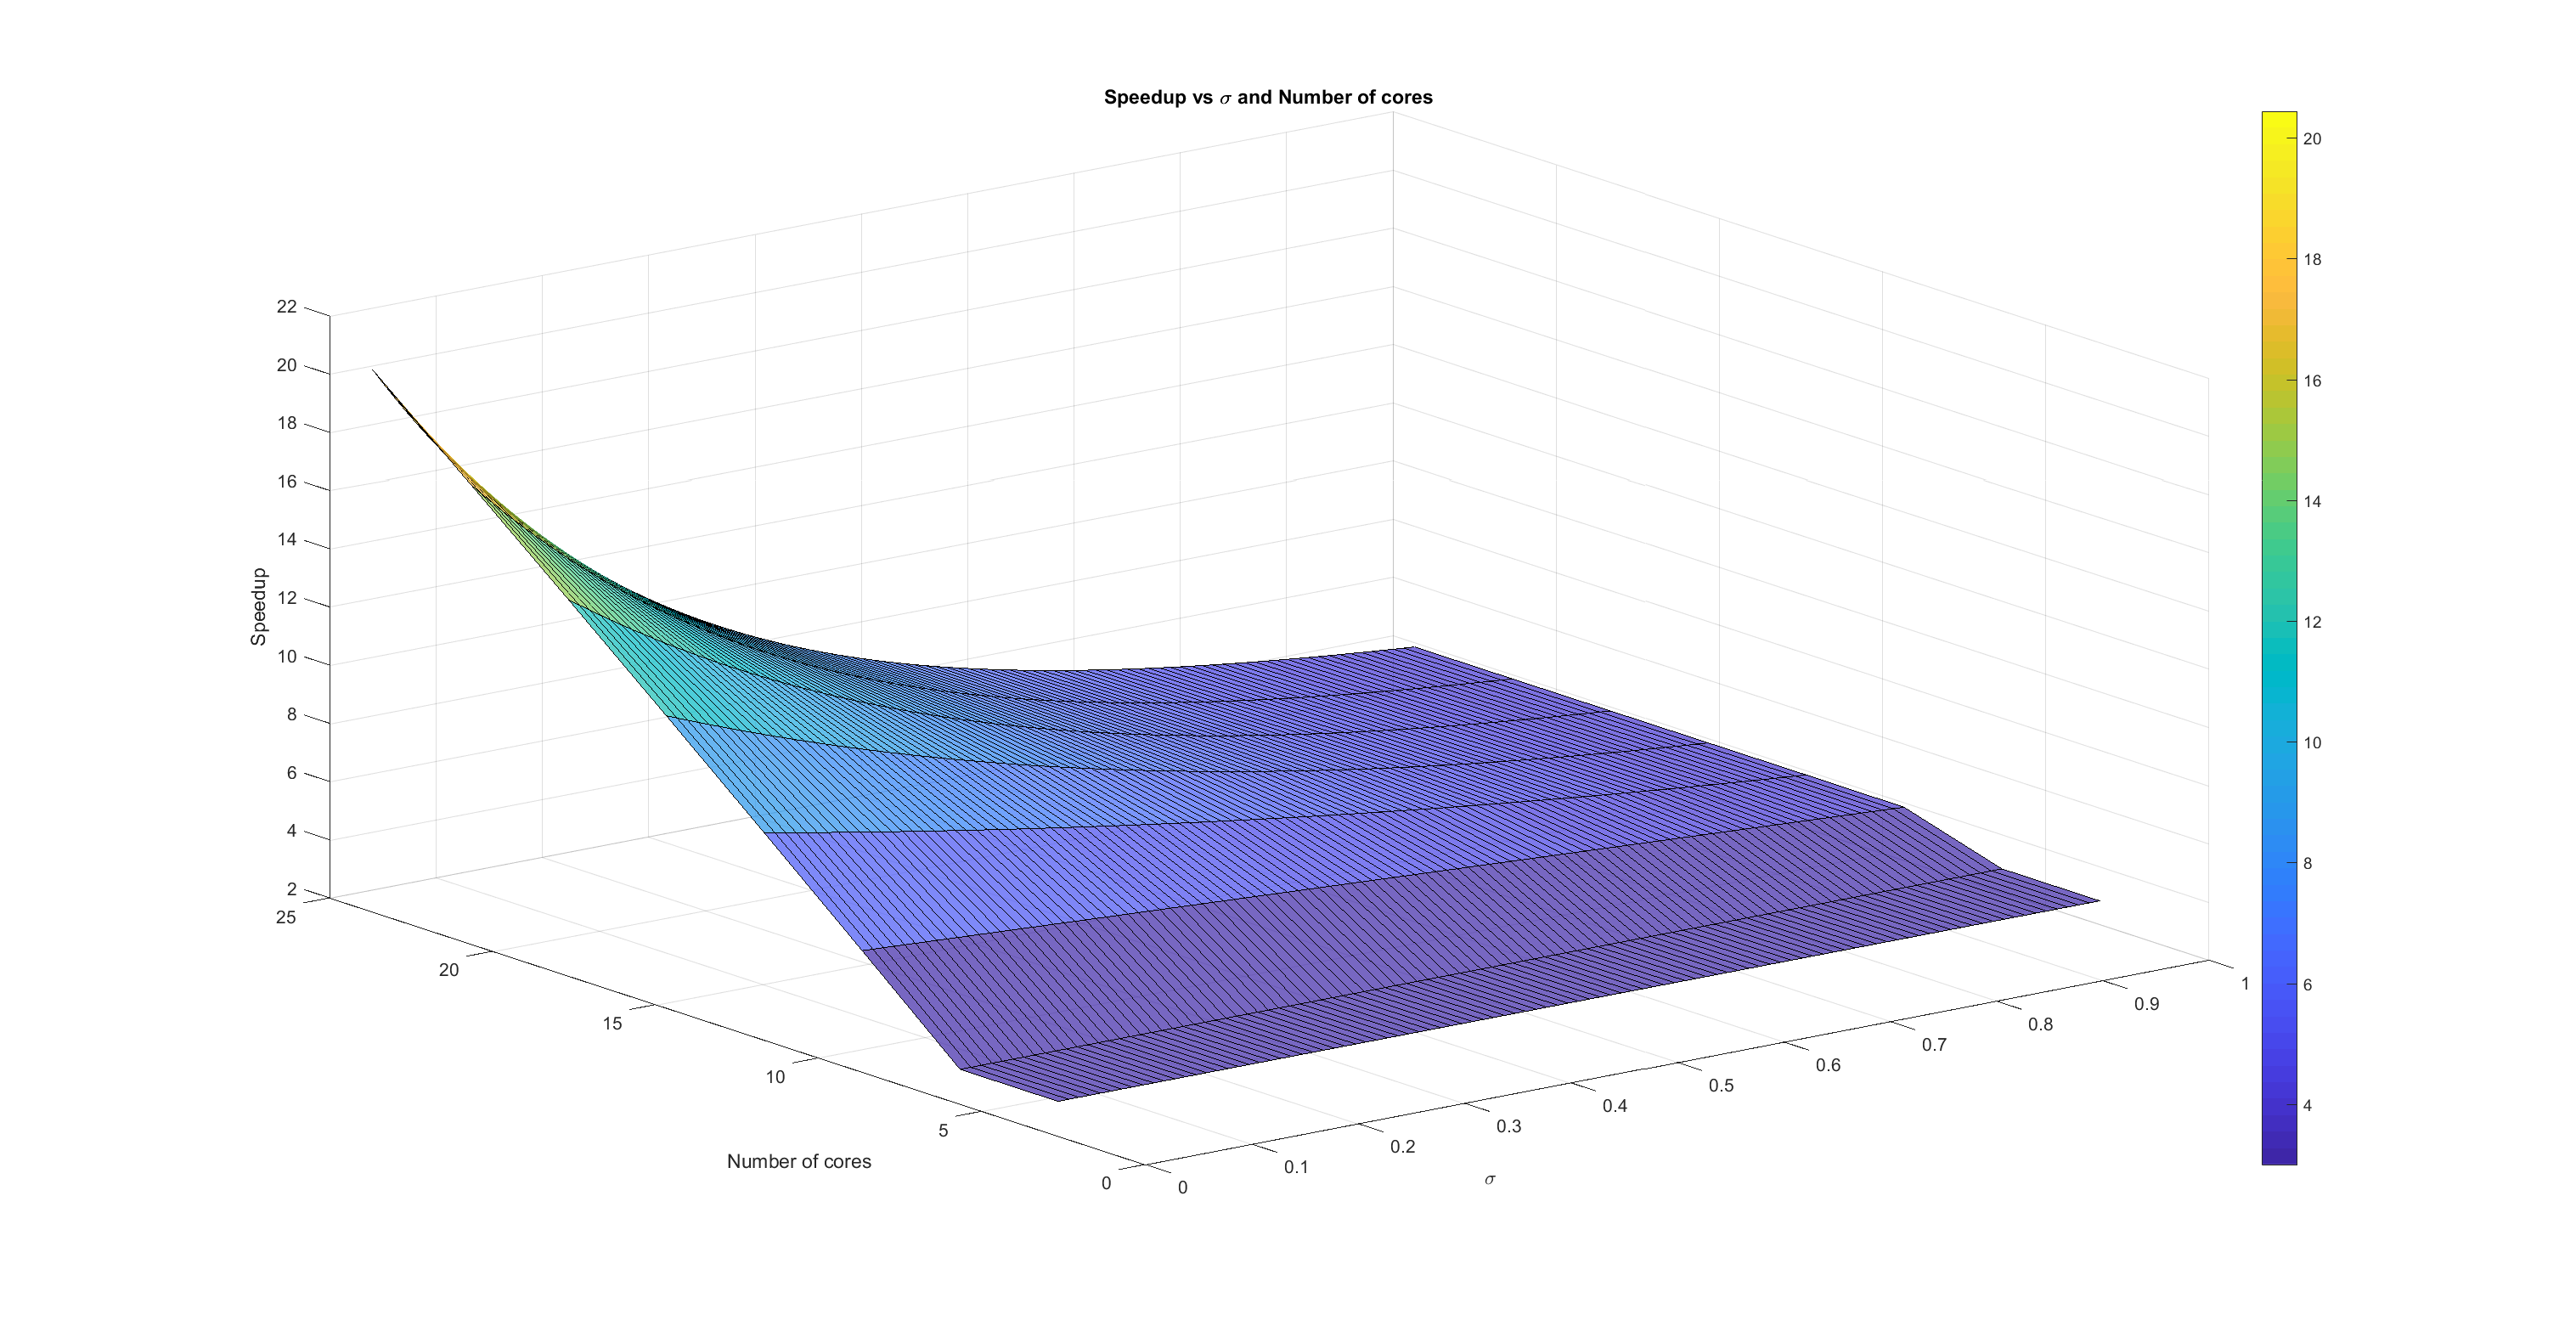
\includegraphics[width=1\columnwidth]{figure/sa3t8b.eps}
\caption{Sensitivity analysis result of 3*8 regular network and the injection position on boundary processor $P_{2}$}
\label{fig:sa3t8b}
\end{figure}
\Fig{sa3t8b} shows that if the value $\sigma > 0.2$, the speedup simulation effect is obvious.   If the value $\sigma < 0.1$, the number of cores has linear impact on the speedup performance.   If the number of cores $>$ 5, the bottom effect with front-end, the cluster at least get about $4$ times speedup.   The reason is $P_{0}$ has $3$ $level_{1}$ processors.  

\newpage

\subsubsection{Data Injection On The Inner Grid Processor}
\Fig{5t5}, $L$ incurs on $P_{12}$ and the simulation result says:
\begin{figure}[!ht]
\centering
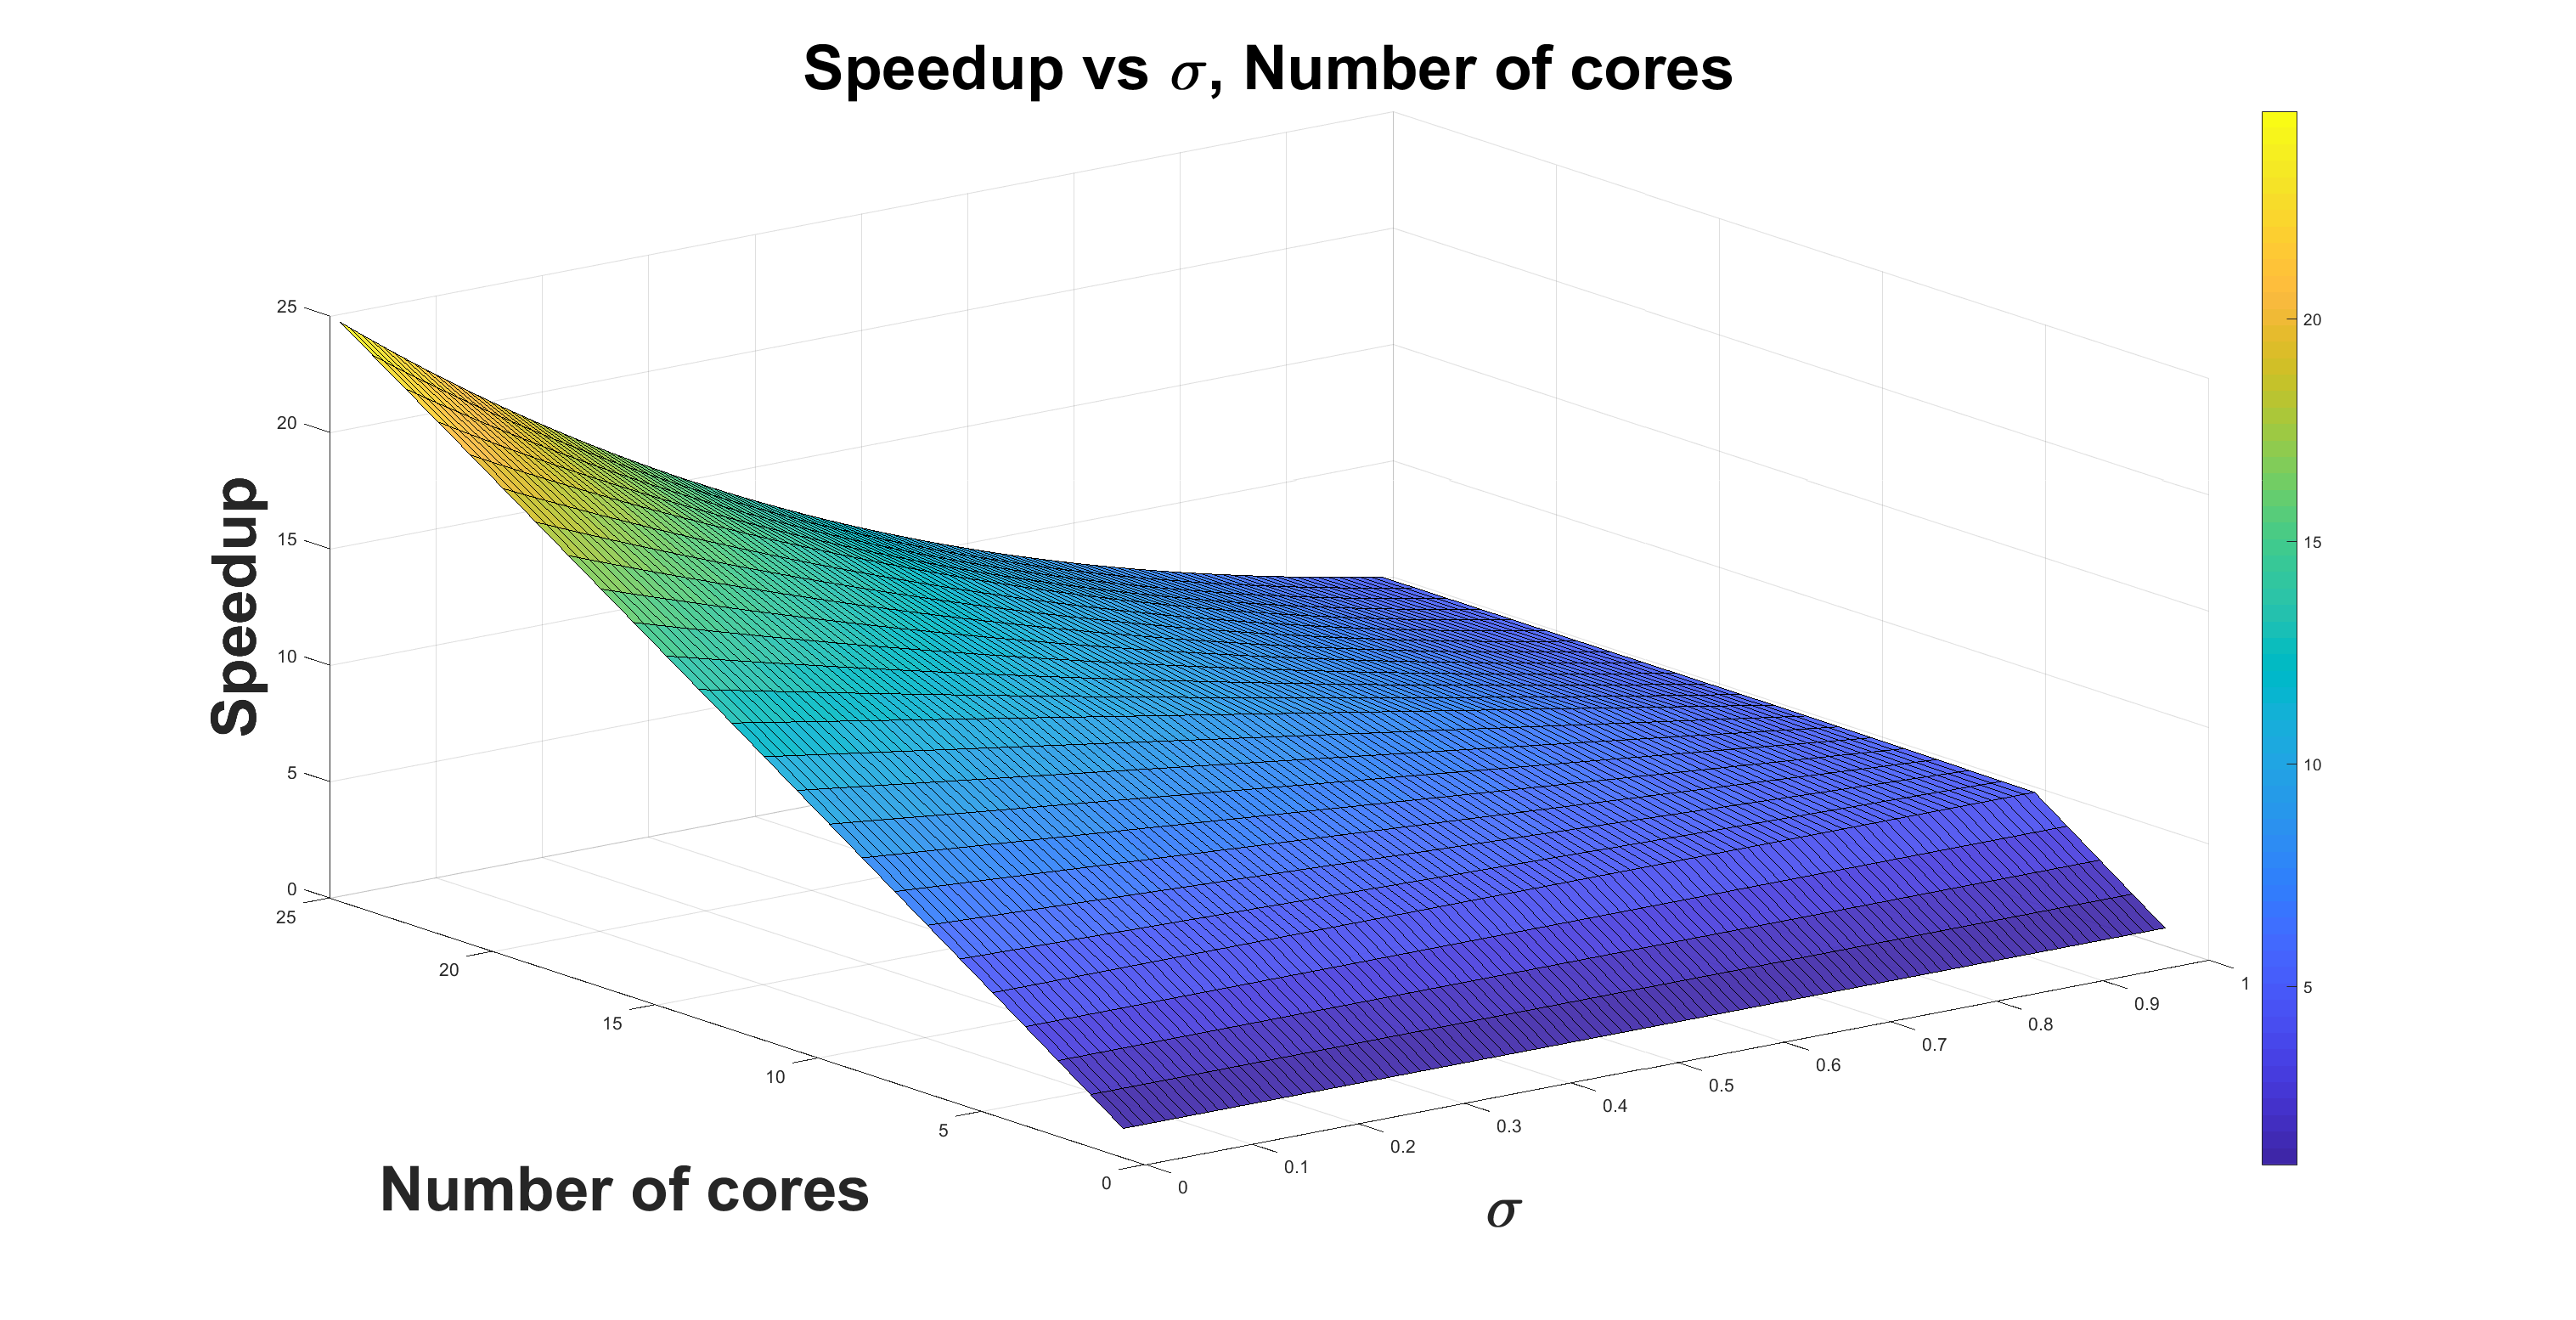
\includegraphics[width=1\columnwidth]{figure/sa5t5i.eps}
\caption{Sensitivity analysis result of data injection position on inner grid processor}
\label{fig:sa5t5i}
\end{figure}
If the number of processor large than $5$, the cluster equivalence computation ability is at least $5$ time speedup.  It is the inner grid has $4$ $level_{1}$ neighbor processors.  
\newpage
